\section{Introduction}
Reasoning with paths over user-item associated Knowledge Graphs (KGs) has been becoming a popular means for explainable recommendations \cite{xian2019reinforcement, wang2019explainable, zhao2020leveraging}. The path-based recommendation systems have successfully achieved promising recommendation performance, as well as appealing explanations via searching the connectivity information between users and items across KGs. One category of existing works on path-based explainable recommendations seeks auxiliary meta-paths (pre-defined higher-order relational compositions between various types of entities in KGs) as similarity measures and evidence for possible explanations between users and items. 

However, most of existing path-based methods for explainable recommendation simply treat the underlying KGs as static graphs, ignoring the dynamic and evolving nature of user-item interactions in real-world recommendation scenarios. The dynamics and evolutions of users' interactions with items play a pivotal role in both recommendation precision and explanations for a users' real intent. Take the scenario in Figure \ref{fig:1} as an example, Alice purchased a phone case and a phone film after a recent buy of a new phone. If we ignore the sequential information between each purchase (in Fig \ref{fig:1-1}) and treat the whole information as a static graph (in Fig \ref{fig:1-2}), the system probably gives an explanation of buying the phone case is because a similar customer also bought this phone case by exploring co-purchasing relationships. Whilst the explanation, in this case, might be valid and the underlying reasoning mechanism (collaborative filtering signal) can be used for recommendation, it is still sub-optimal as a more appealing motivation of buying a phone case is due to the recent purchase of a new phone. For this reason, in this example, it is important for a system to be capable of considering temporal and sequential user-item interactions and disentangling the importance of various reasons when generating possible explanations. 
% \begin{figure}[ht]
% 	\vspace{-0.35cm}
% 	
\includegraphics[scale=0.274]{figs/figure1.pdf}
% 	\caption{The concept of TEMR-RL. TEMR-RL contributes a sequential dynamic modelling layer on top of existing knowledge-aware explainable recommendation (the dashed box on the bottom).} \label{fig:1}
% 	\vspace{-0.4cm}
% \end{figure}


\begin{figure}
\begin{subfigure}{.5\textwidth}
  \centering
  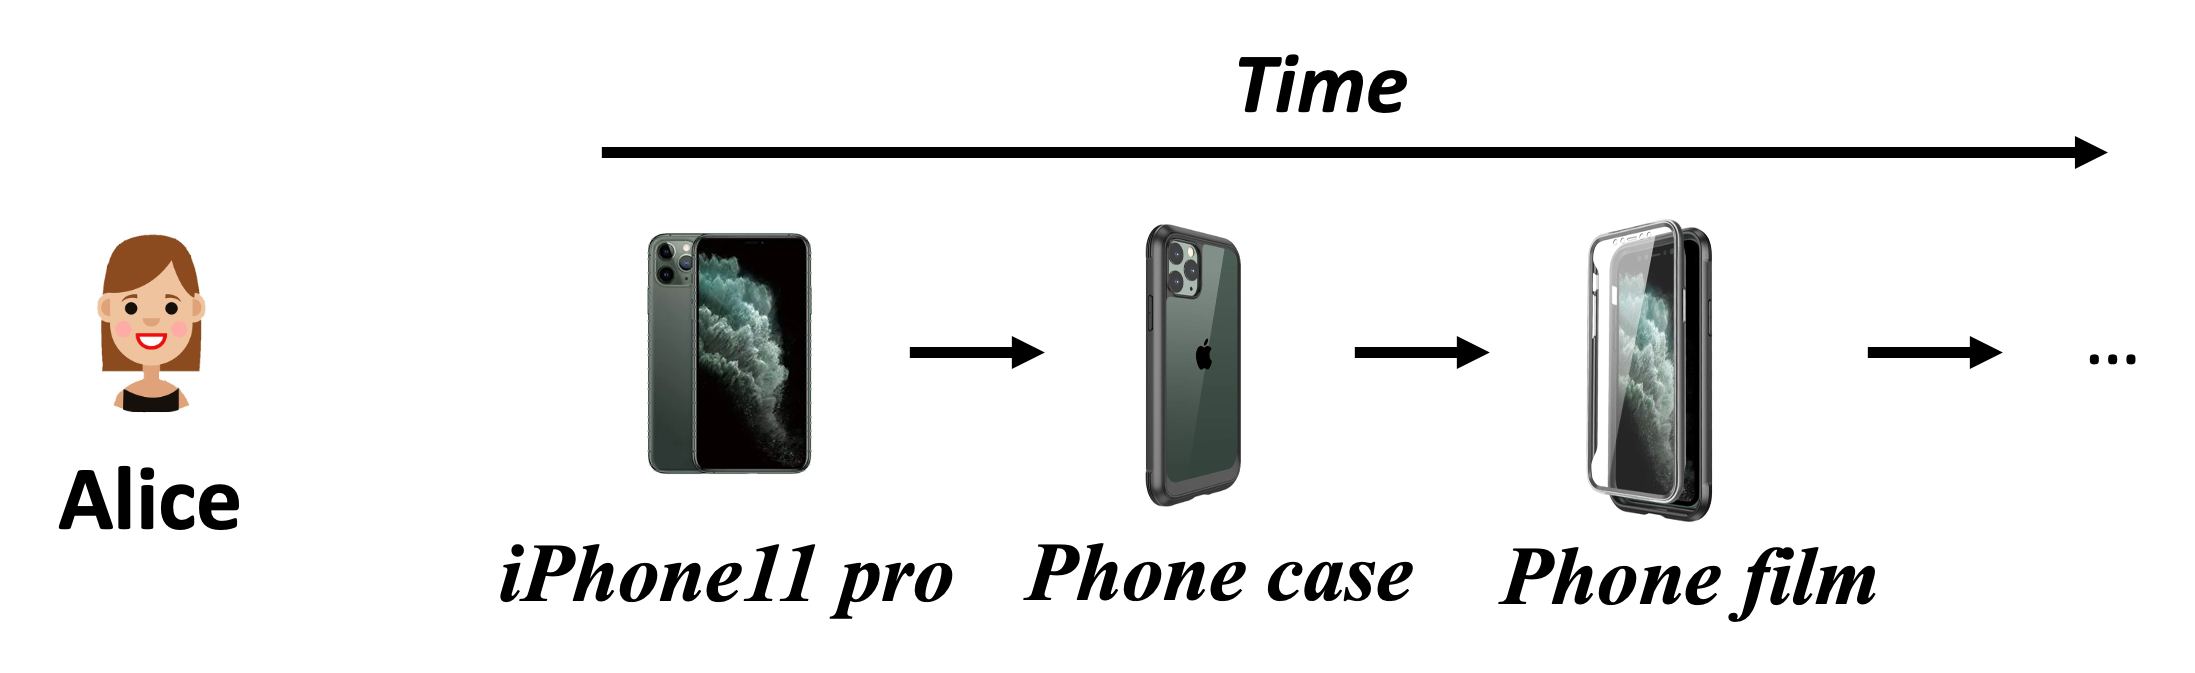
\includegraphics[scale=0.4]{figs/fig1_1_notitle.png}  
  \vspace{-0.5em}
  \caption{Intuitive sequential modelling}
  \label{fig:1-1}
\end{subfigure}

\vspace{1.5em}

\begin{subfigure}{.5\textwidth}
  \centering
  
  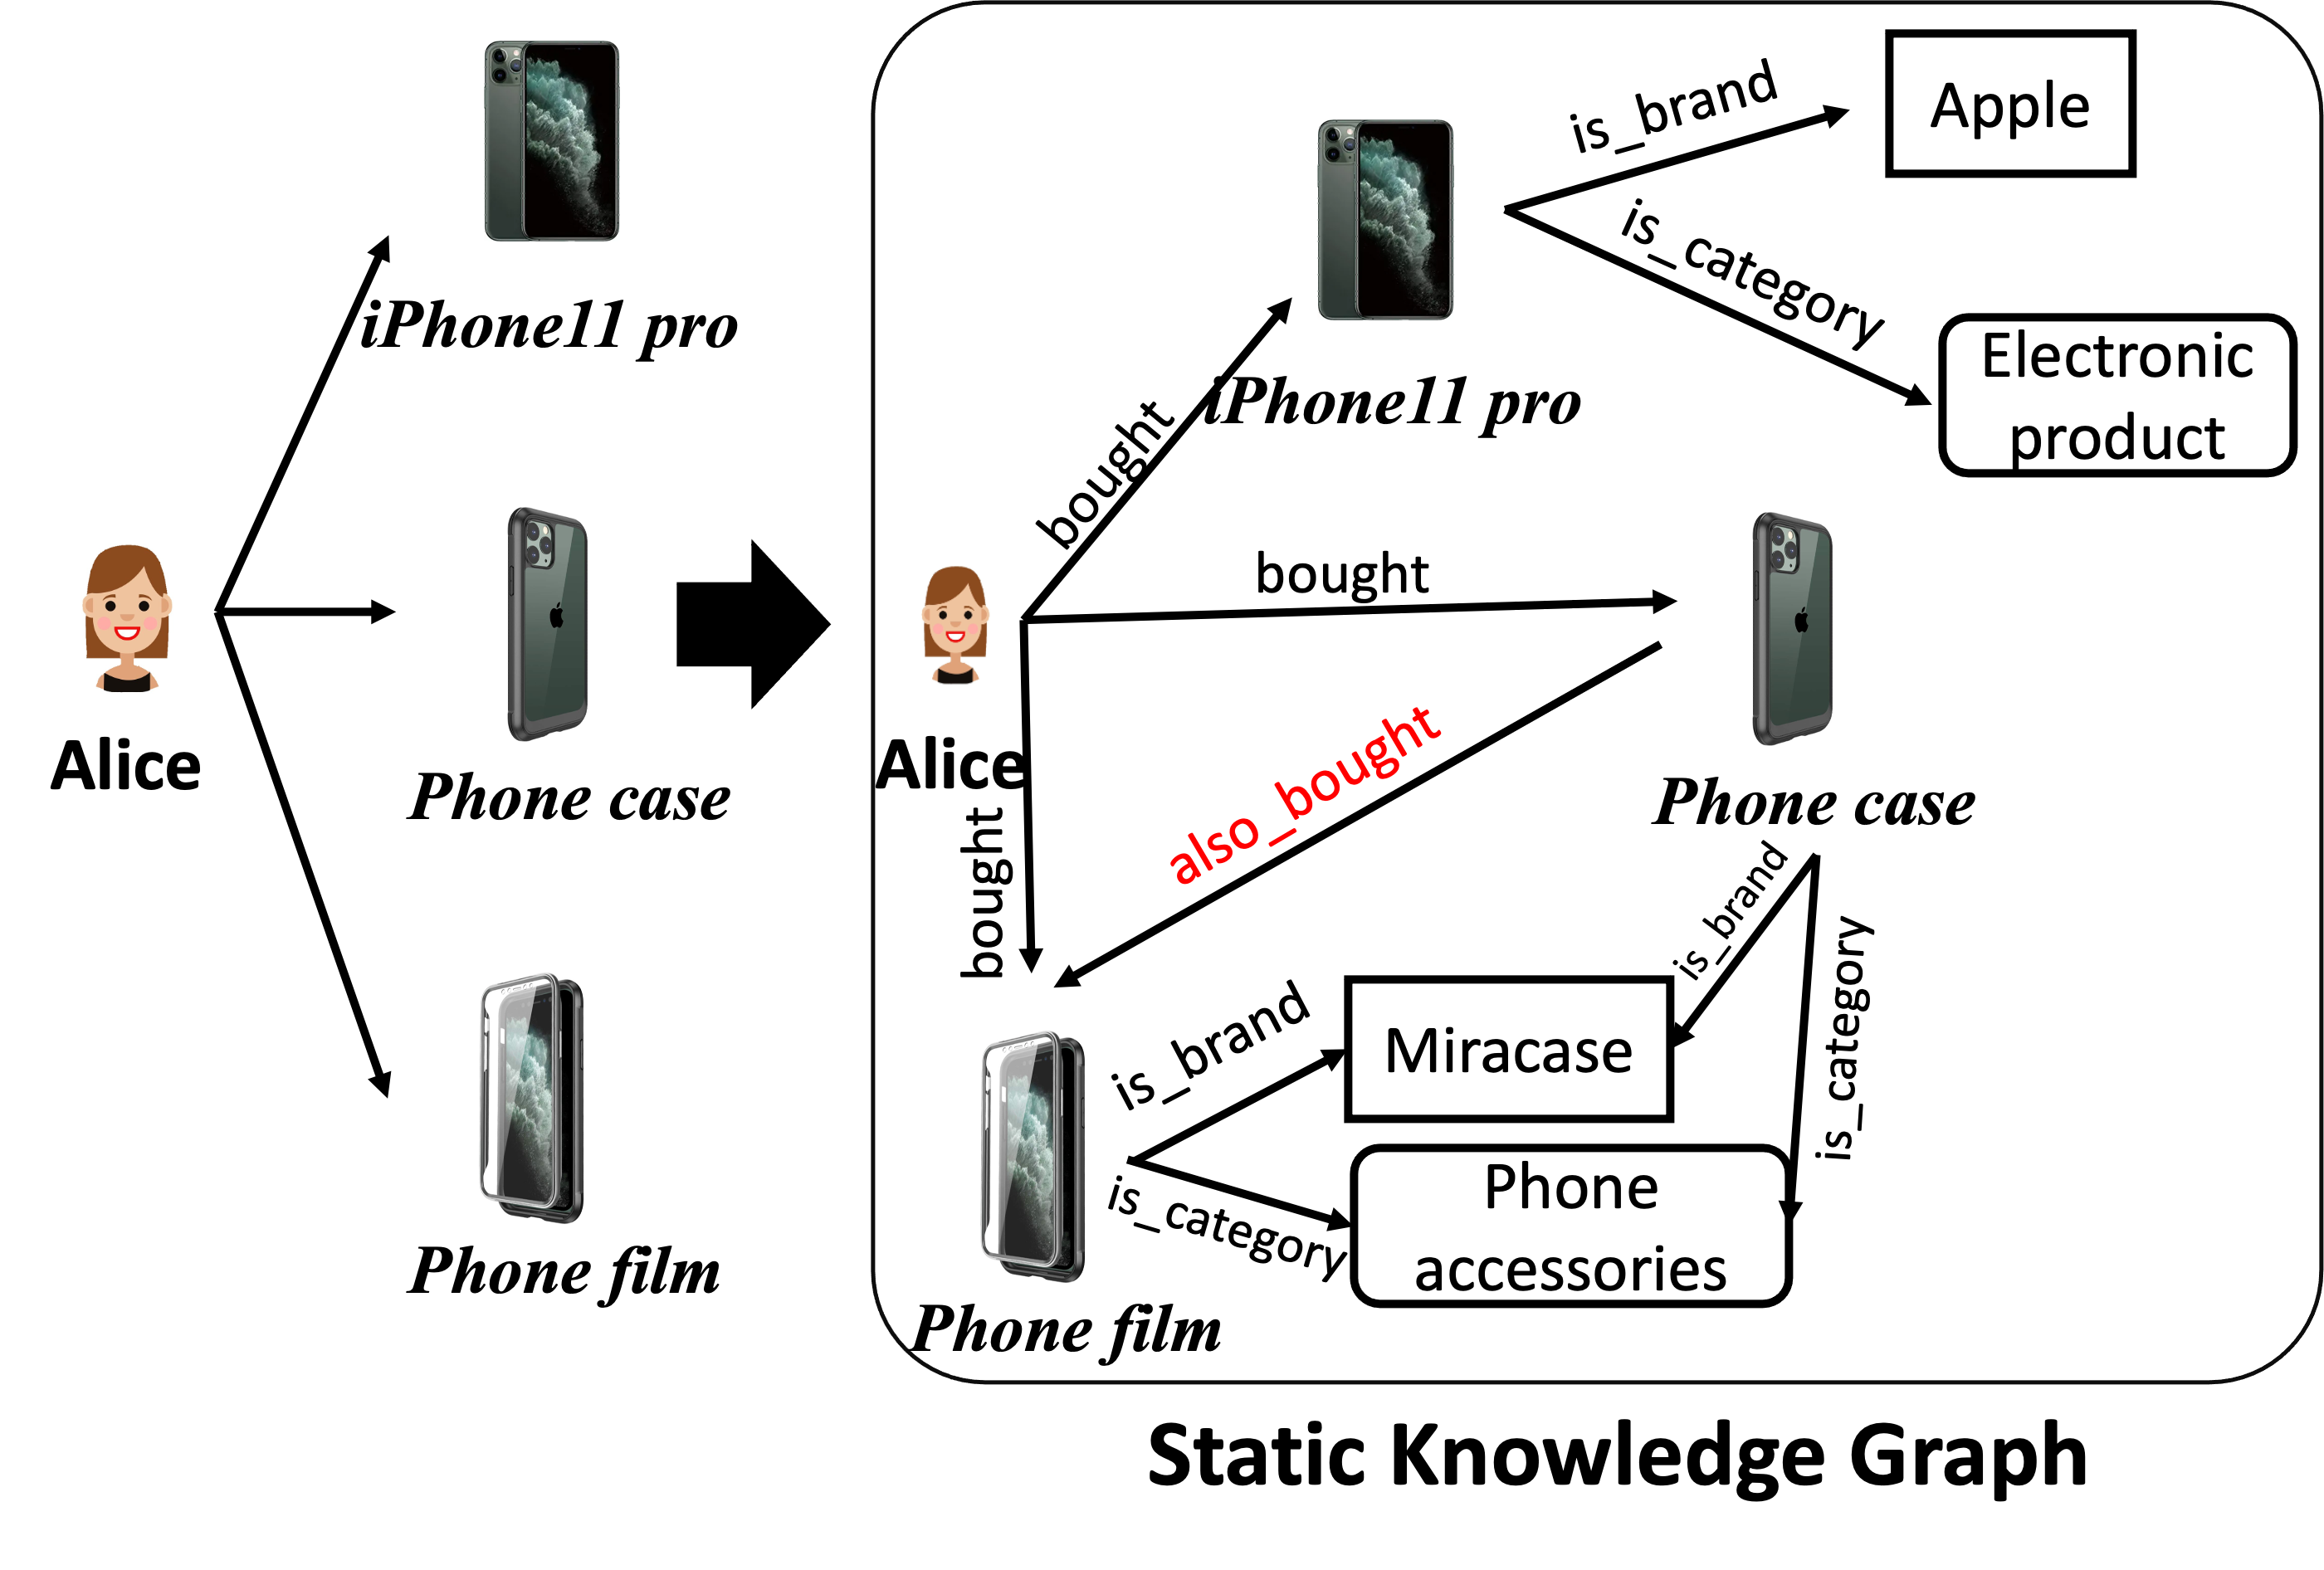
\includegraphics[scale=0.4]{figs/fig1_2_notitle_update.png}  
  \vspace{-0.5em}
  \caption{Existing static knowledge-graph based modelling}
  \label{fig:1-2}
\end{subfigure}

\caption{Existing Sequential modelling and static knowledge-graph based modelling.}
\label{fig:1}
\end{figure}

Although some prior works have considered some extent of the sequential information for knowledge-aware path-based explainable recommendation problem, they still fail to explicitly model the dynamics of users' activities. To allow effective reasoning on paths to infer the underlying rationale of a user-item interaction, the method proposed in \cite{wang2019explainable} takes the advantages of path connectivity and leverages the sequential dependencies of entities and sophisticated relations of a path connecting a user-item pair. Nevertheless, the methods only consider the sequential information within specific paths and did not consider the importance of the user' historical sequences on reflecting the user's dynamic interactions with items. To improve, the KARN model \cite{zhu2020knowledge} fuses the user's clicked history sequence and path connectivity between users and items in KGs for recommendation. However, the method models the user's sequential behaviours and user-item interactions separately and in a coarse-grained manner (treating a user's click history as a whole), which may restrict the expressiveness of users' temporal dynamics on recommendation explainability. 

In light of this, in this paper, we challenge the problem of exploring users' temporal sequential dynamics in the context of path-based knowledge-aware recommendation. Different from existing works that either only consider the sequential information within a path or treat the user's sequential interactions as a whole and separately, we aim to 1) explicitly model and integrate the dynamic user-item interactions over time into the path-based knowledge-aware recommendation, and 2) leverage the captured dynamics of user-item interactions to improve the performance and explainability of the recommendation.

It is worth noting that modelling users' temporal sequential behaviour with path-based knowledge-aware explainable recommendation is a non-trial and challenging task. First, path-based knowledge-aware recommender systems are built upon the well-constructed KGs, and its expected accuracy and explainability are highly related to the underlying KGs and distilled paths. If temporal information between users and items is considered, the original underlying static KGs will be cast into multiple snapshots w.r.t. the timestamps. Comparing with the static KGs that consist of all users' full timelines, each snapshot at a certain timestamp only has partial observations of the global knowledge, which will result in inferior recommendation performance. To deal with the issue, we devise a general framework for temporal knowledge aware reinforcement path-based explainable recommender systems, namely \textbf{Temporal Meta-path Guided Explainable Recommendation leveraging Reinforcement Learning (TMER-RL)}. TMER-RL provides a solution that can explicitly depict users' sequential behaviour while being able to be aware of global knowledge of the entire underlying KGs. Specifically, to model the temporal dynamics between users and items, TMER-RL naturally models the task as a sequential recommendation problem and takes as input users and their corresponding sequential purchase history. To learn the sequential dependencies between consecutive items purchased by a user, TMER-RL novelly explores item-item paths between consecutive items and embed the paths as context with elaborated designed attention mechanisms to model the dynamics between user and items. Compared to existing path-based explainable recommendation systems that only consider user-item paths as evidence and support for the recommendation decision, TMER-RL contributes another creamy layer on the top of existing works, which makes use of the powerful expressiveness of temporal information between users and items. 



In addition, when taking paths into consideration for the above purpose, another challenge lies in the existence of a large number of possible paths. It is time-consuming for a model to select several paths that are meaningful, expressive, and have positive impacts on both recommendation performance and explainability.
To this end, inspired by prior work \cite{hu2018leveraging}, our previous work TMER \cite{10.1145/3437963.3441762} leverages the concept of meta-path \cite{sun2011pathsim} and explore diverse meta-path schemas to characterize the context of dynamic interactions between users and items. However, it has to pre-define meta-paths and randomly sample path instances from all generated ones, which involves human and random factor in the following recommendation module. To explore paths effectively, we utilize reinforcement learning with our designed useful score function for paths to mine diverse meta-path instances. With resort to the powerful transformer model for sequential modelling, we also elaborate item-item path attention and user-item path attention units to learn combinational features of multiple paths to further characterize users' temporal purchasing motivations and their general shopping tastes, respectively. The rationale for developing such path-based attention units is that a user's motivation towards buying a certain product is complex and consists of multiple factors. For example, when buying a new phone, a customer may consider several factors including a phone's intrinsic features such as functionality, display, camera, etc., as well as other external factors such as the choices of their close friends, and their previous purchase of certain related electronics using the same operating system. With help of the designed path-based attention units, the proposed TMER-RL framework is able to learn different weights for various possible paths which will be then used as explanations for recommendations (we show the effectiveness of using the proposed path-based attention units for the explainable recommendation in the experiments by running case studies). 

Another shining point of our work is that the introduced item-item path modelling also serves as the core of the simple yet effective sequential modelling architecture of TMER-RL. The combinational meta-path enriched features learned by the item-item path attention units are aggregated with features of previous purchased item will serve as the prediction signals for the next item. The intuition behind is that the item-item paths connect two consecutive items purchased by a user, and represent various reasons and factors that may lead to the next purchased item, which intrinsically provides strong sequential dependencies between items. Compared to existing works on the sequential recommendations that rely on Recurrent Neural Nets such as (RNNs\cite{liu2016context}, GRUs\cite{hidasi2018recurrent}, LSTM\cite{wang2019explainable, zhu2020knowledge}), the proposed methods in this paper is light, simple but effective. 


The main contributions of this paper are summarized as follows:
\begin{itemize}
	\item We point out that explicitly modelling dynamic user-item interactions over time can significantly benefit the recommendation performance and explainability. We introduce, to the best of our knowledge, the first study to model users' temporal sequential behaviour with path-based knowledge-aware explainable recommendation.
	
	\item We propose \textbf{T}emporal \textbf{M}eta-path Guided \textbf{E}xplainable \textbf{R}ecommendation leveraging \textbf{R}einforcement \textbf{L}earning (\textbf{TMER-RL}), which considers users' dynamic behaviours on top of the global knowledge graph for sequential-aware recommendation and explores both user-item and item-item meta-path paths with well-designed reinforcement framework and attention mechanisms for explainable recommendation.
	
	
	\item Extensive evaluations on three real-world benchmark datasets have been conducted, and the experimental results demonstrate the superiority, effectiveness and temporal explainability of the proposed TMER-RL model. 
	
\end{itemize}